\subsection{Überblick}
Zur Koordination der Abläufe, sowie der Erkennung des Korbes wurden zwei verschiedene Applikationen entwickelt. Einerseits eine Viewer-Applikation, über welche der Ballwerfer konfiguriert und gestartet wird und die erhaltenen Rückgabewerte ausgegeben werden. Des weiteren wurde eine Smartphone-App entwickelt. In dieser Applikation werden die Hauptfunktionalitäten wie beispielsweise die Korberkennung ausgeführt. Der Viewer wird auf einem beliebigen Endgerät wie etwa einem Laptop ausgeführt, wobei die Smartphone-App auf einem Smartphone läuft, welches direkt an der Front des Ballwerfers befestigt wird. Die beiden Applikationen werden via WLAN verbunden und kommunizieren über diese Schnittstelle mittels Data Transfer Objects (DTOs). Die einzelnen Komponenten können im abgebildeten Kontextdiagramm entnommen werden.\ref{abb:Kontextdiagramm}

\begin{figure}[h!]
	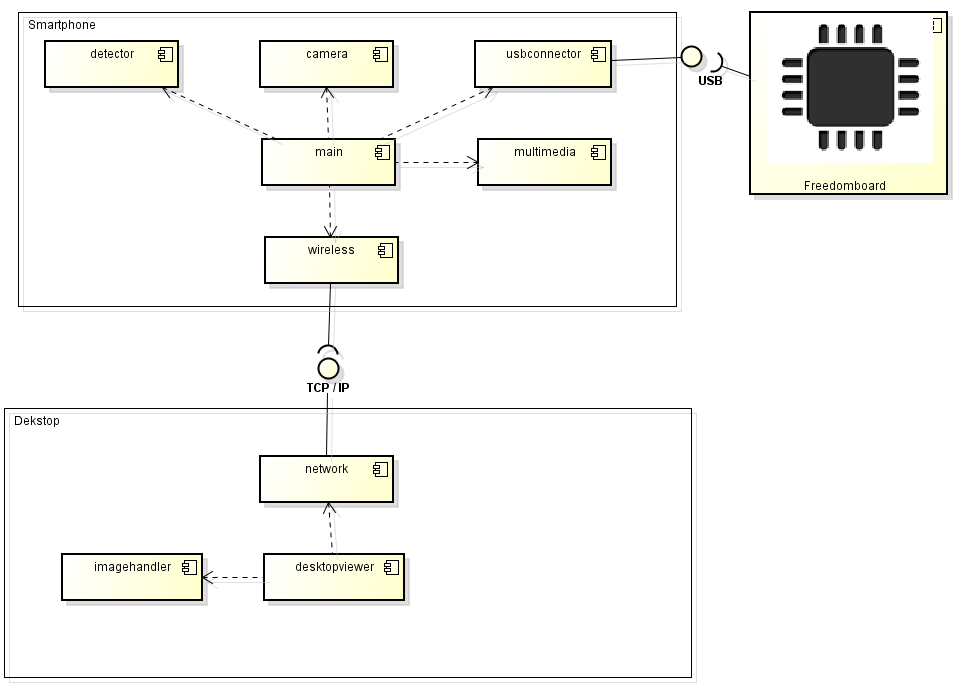
\includegraphics[width=1\textwidth,clip,trim=4mm 0mm 15mm 0mm]
	{Enddokumentation/Bilder/KontextDiagramm_PREN2_v2.png}
	\centering
	\caption{Übersicht Komponenten}
	\label{abb:Kontextdiagramm}
\end{figure}

\begin{figure}[h!]
	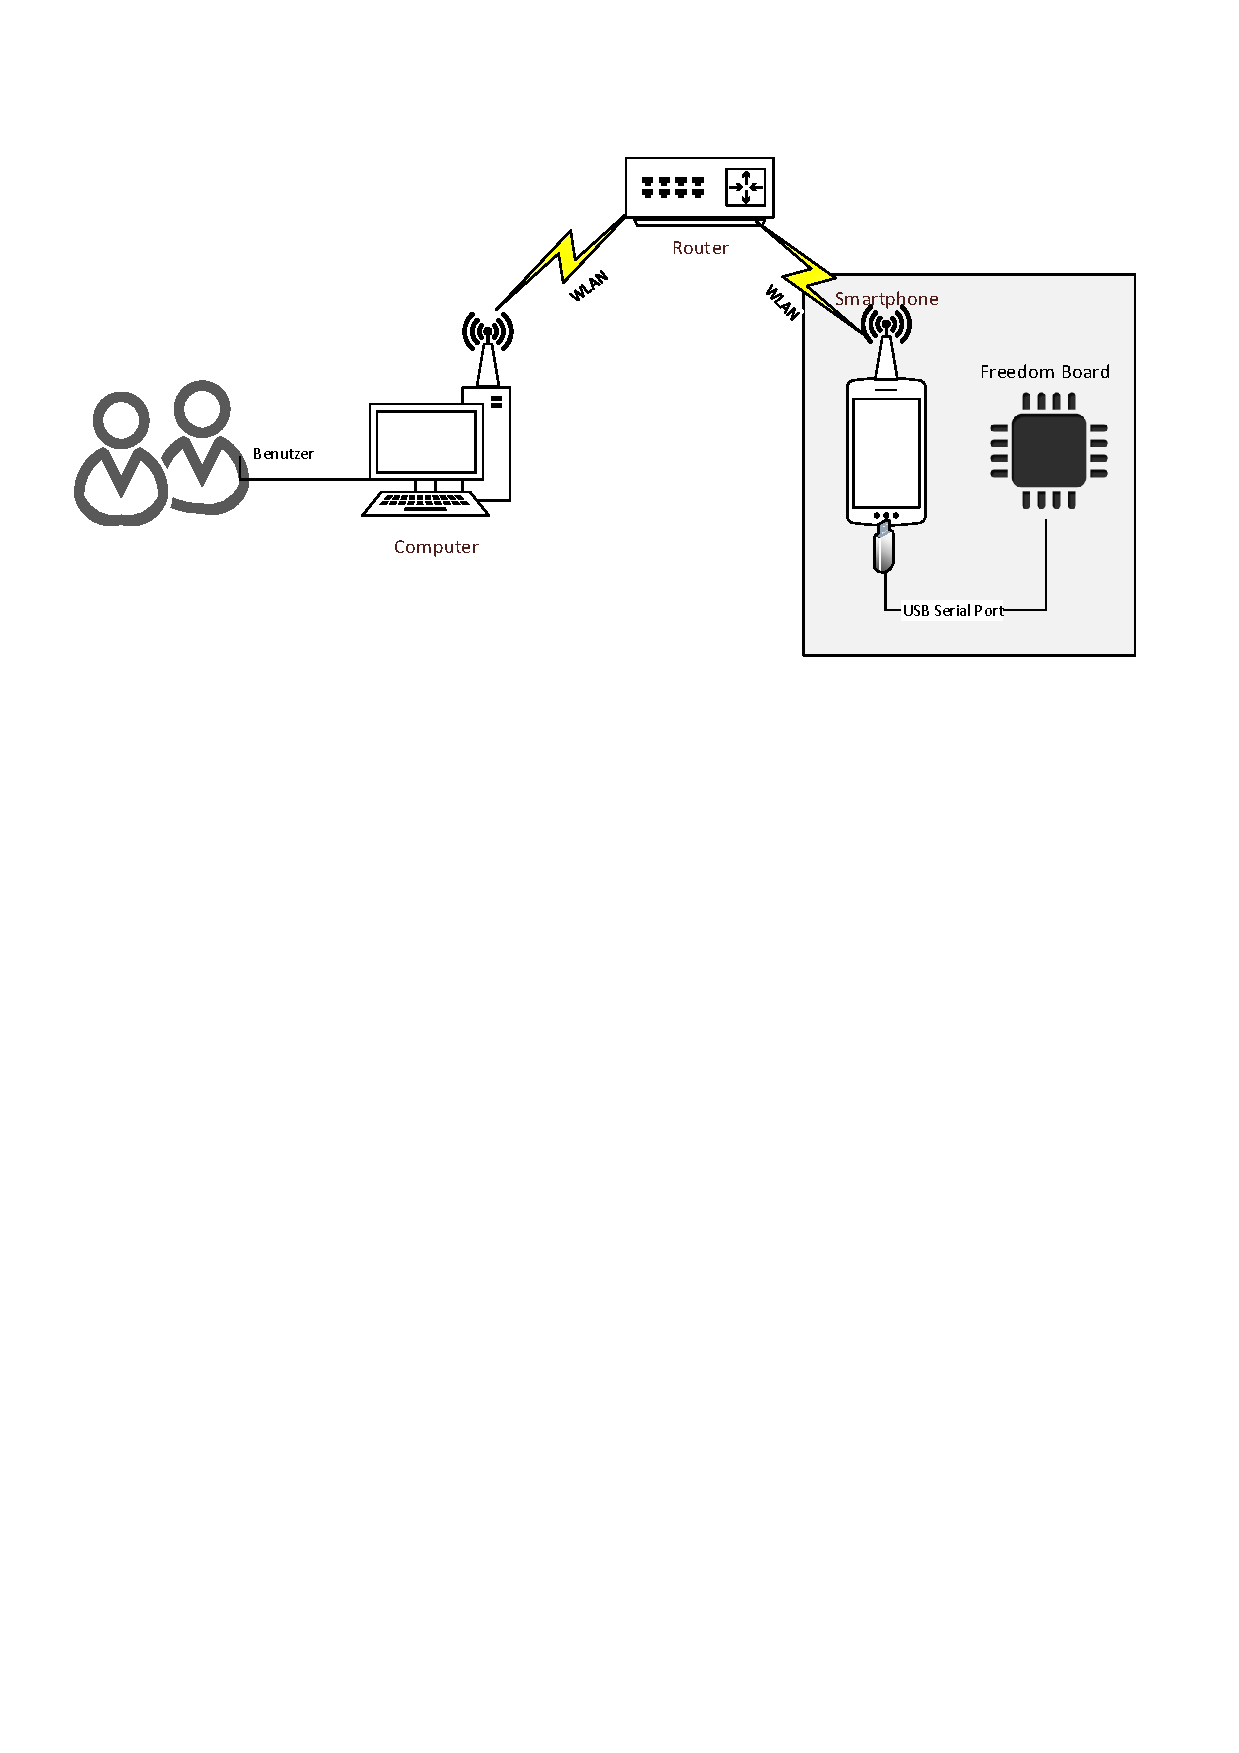
\includegraphics[width=0.8\textwidth,clip,trim=12mm 180mm 15mm 20mm]
	{Enddokumentation/Bilder/Kommunikation_PREN2_v1.pdf}
	\centering
	\caption{Übersicht der beteiligten Geräte}
	\label{abb:UebersichtKommunikation}
\end{figure}
